\documentclass{beamer}

% Packages
\usepackage{graphicx}    % For including images
\usepackage{amsmath}     % For mathematical symbols
\usepackage{braket}      % For Dirac notation
\usepackage[absolute,overlay]{textpos}
\usepackage{amsmath}
% \usepackage{amsmath, amssymb, dsfont}
% \usepackage{algorithm}
% \usepackage{algorithmicx}
% \usepackage{enumitem}


\theoremstyle{definition}
\newtheorem{algorithm}{Algorithm}
\newtheorem{construction}[theorem]{Construction}

\newcommand\numberthis{\addtocounter{equation}{1}\tag{\theequation}}

\newcommand{\cas}{\mathrm{cas}}
\newcommand{\cht}{\mathsf{H}}
\newcommand{\qht}{\mathsf{QHT}}
\newcommand{\cft}{\mathsf{F}}
\newcommand{\qft}{\mathsf{QFT}}
\newcommand{\comph}{\mathsf{cmpIndex}}
\newcommand{\gen}{\mathsf{Gen}}
\newcommand{\ver}{\mathsf{Ver}}




% Title Information
\title{Quantum Walks and Applications to Quantum Money}
\author{Seyed Ali Mousavi}
\institute{Supervised by Dr. Jake Doliskani}
\date{\today}

\begin{document}

% Title Slide
\begin{frame}
    \titlepage
\end{frame}





% \begin{frame}{Program and Courses Taken}

   
    
%     \begin{textblock*}{12cm}(0.5cm,1.5cm)
%        \begin{itemize}
%         \item Program: M.A.Sc in Software Engineering
%         \vspace{1cm}
%         \item CAS 701,  Logic \& Discrete Mathematics
%         \item COMPSCI 6TE3, Continuous optimization
%         \item CAS 721, Combinatorics \& Computing
%         \item CAS 741, Development of Scientific Computation Software
%        \end{itemize}
%     \end{textblock*}

%     \title{SDSD}
    


% \end{frame}







% \begin{frame}{Seminars}
    
%     \begin{textblock*}{12cm}(0.5cm,1.5cm)
%        \begin{itemize}
%         \item I have participated in 6 seminars during my program.
%        \end{itemize}
%     \end{textblock*}
    

% \end{frame}




% \begin{frame}{Poster}
    
%     \begin{figure}
%         \centering
%         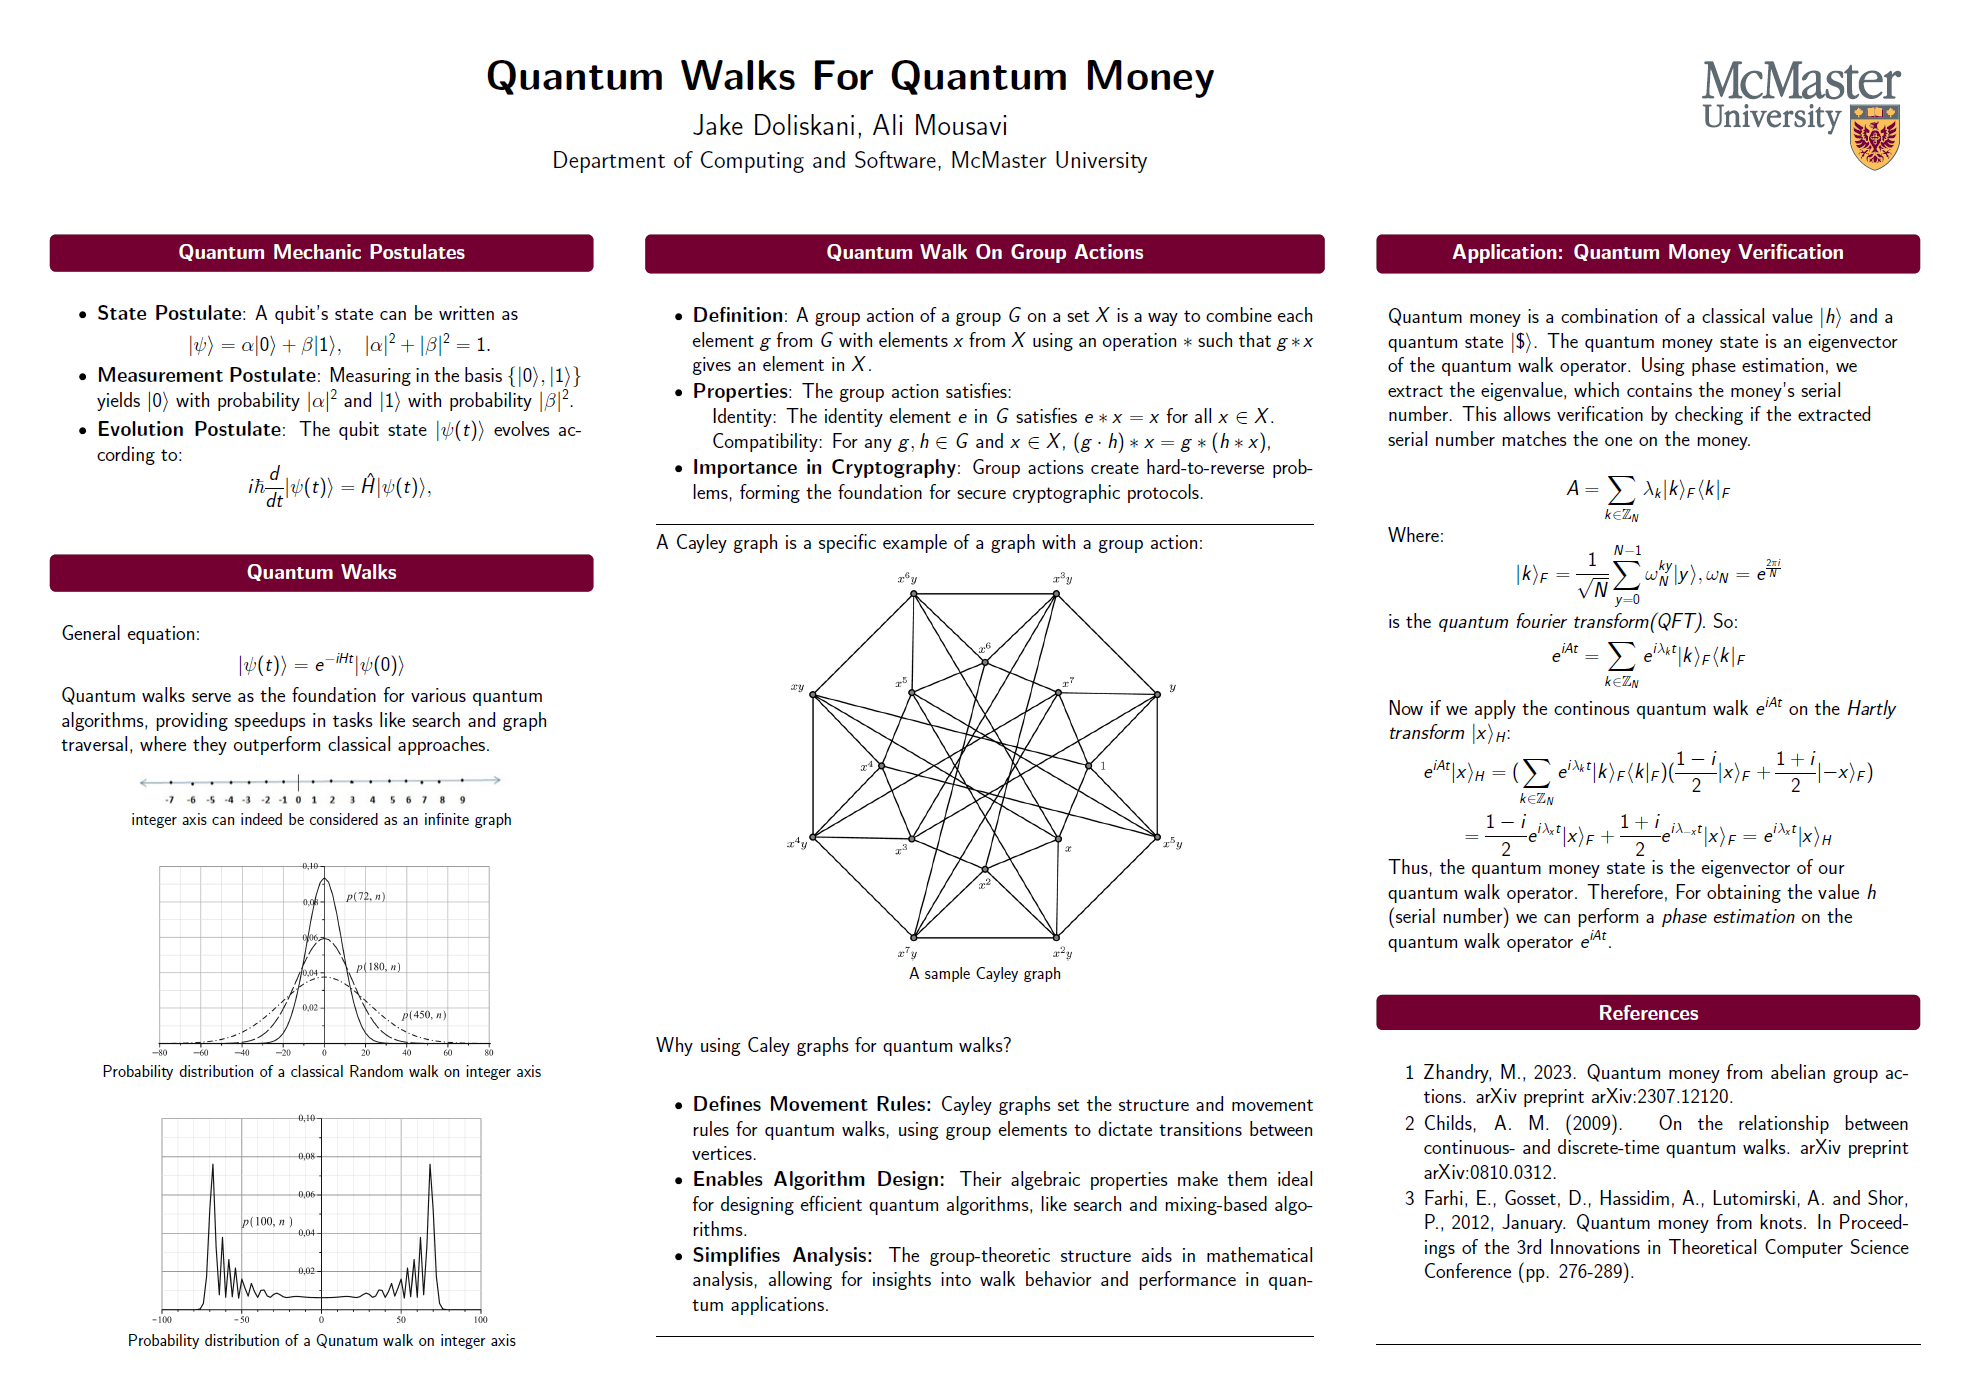
\includegraphics[width=1\textwidth]{poster.png}
%         \caption{Presented at Nov. 6, 2024}
%     \end{figure}

% \end{frame}




\begin{frame}{Quantum Computation - Preliminaries and Notation}
    
    \begin{textblock*}{12cm}(0.5cm,1.5cm)
        \begin{itemize}
            \item Consider a finite Hilbert space $\mathcal{H}$ with an orthonormal set of basis states $\{ \lvert s_i \rangle \}$ for $s \in \mathcal{S}$. The states $s \in \mathcal{S}$ may be interpreted as the possible classical states of the system described by $\mathcal{H}$. \\
            \vspace{1cm}
            \item In general, the state of the system, $\lvert \alpha \rangle$, is a unit vector in the Hilbert space $\mathcal{H}$ and can be written as $\lvert \alpha \rangle = \sum_{s \in \mathcal{S}} a_s \lvert s \rangle$, where $\sum_{s \in \mathcal{S}} |a_s|^2 = 1$. \\
            \vspace{1cm}
            \item $\langle \alpha \rvert$ denotes the conjugate transpose of $\lvert \alpha \rangle$. The expression $\langle \beta \rvert \alpha \rangle$ denotes the inner product of $\lvert \alpha \rangle$ and $\lvert \beta \rangle$.

        \end{itemize}
            
    \end{textblock*}
\end{frame}




\begin{frame}{Quantum Computation - Quantum Postulates}
    
    \begin{textblock*}{12cm}(0.5cm,1.5cm)
        \begin{itemize}
            \item \textbf{Unitary evolution}: Quantum physics requires that the evolution of quantum states is unitary; that is, the state $\lvert \alpha \rangle$ is mapped to $U \lvert \alpha \rangle$, where $U$ satisfies $U \cdot U^{\dagger} = I$, and $U^{\dagger}$ denotes the conjugate transpose of $U$.
            \vspace{0.5cm}
            \item \textbf{Measurement}: We will describe here only a measurement in the orthonormal basis $\lvert s \rangle$. The output of the measurement of the state $\lvert \alpha \rangle$ is an element $s \in \mathcal{S}$, with probability $|\langle s \vert \alpha \rangle|^2$. Moreover, the new state of the system after the measurement is $\lvert s$.
            \vspace{0.5cm}
            \item \textbf{Combining two quantum systems}: If $\mathcal{H}_A$ and $\mathcal{H}_B$ are the Hilbert spaces of two systems, $A$ and $B$, then the joint system is described by the tensor product of the Hilbert spaces, $\mathcal{H}_A \otimes \mathcal{H}_B$. If the basis states for $\mathcal{H}_A$ and $\mathcal{H}_B$ are $\{ \lvert a_i \rangle \}$ and $\{ \lvert v_i \rangle \}$ respectively, then the basis states of $\mathcal{H}_A \otimes \mathcal{H}_B$ are $\{ \lvert a_i \rangle \otimes \lvert v_i \rangle \}$.


            
        \end{itemize}
            
    \end{textblock*}
\end{frame}






\begin{frame}{Quantum Walks}
    
    \begin{textblock*}{12cm}(0.5cm,1.5cm)

        \begin{itemize}
            \item Quantum walks are quantum analogs of classical random walks and play
            a fundamental role in quantum algorithms
            \item  Two types: continuous-time and discrete-time
            \item Quantum walks leverage interference to explore graphs more efficiently than classical walks
            \item For a graph $\Gamma$, a continuous-time classical walk on $\Gamma$ is:
            \[
            \frac{d}{dt} q(t) = Lq(t)
            \]
            \item In the quantum setting,  the dynamics of the walk is given by the Schr\"{o}dinger equation:
            \[
                i\frac{d}{dt}\ket{\psi(t)} = L\ket{\psi(t)}
            \]
            
        \end{itemize}
            
    \end{textblock*}
\end{frame}




\begin{frame}{Continuous-Time Quantum Walks}
    
    \begin{textblock*}{12cm}(0.5cm,1.5cm)

        \begin{itemize}
            \item The solution to this differential
            equation can be written in closed form as:
            \[
                \ket{\psi(t)} = e^{-iLt} \ket{\psi(0)}.
            \]
            \item In practice, we often (including this work) use the adjacency matrix $A$ of $\Gamma$ as the Hamiltonian of the walk
            
        \end{itemize}
            
    \end{textblock*}
\end{frame}






\begin{frame}{Example of a Continuous Quantum Walk}
    
    \begin{textblock*}{12cm}(0.5cm,1.5cm)

                   
    \end{textblock*}
\end{frame}





\begin{frame}{Discrete-Time Quantum Walks}
    \begin{textblock*}{12cm}(0.5cm,1.5cm)
        \begin{itemize}
           
            
            \item If the $\Gamma$ has $N$ vertices, the discrete time quantum walk on $\Gamma$ is defined by a unitary operator on the finite Hilbert space $\mathbb{C}^N \times \mathbb{C}^N$ as follows:
            \item Define the states:
            \[ \ket{\phi_j} = \frac{1}{\sqrt{\deg(j)}} \sum_{k = 1}^N \sqrt{P_{jk}}\ket{j, k}, \]
            \item project and swap operators:
            \[ \Pi = \sum_{j = 1}^N \ket{\phi_j} \bra{\phi_j}, \quad S = \sum_{j, k = 1}^N \ket{j, k} \bra{k, j}. \]
            \item Then, a step of the quantum walk is defined by the unitary:
             \[
             W = S(2\Pi - 1)
             \]

        \end{itemize}
    \end{textblock*}
\end{frame}




\begin{frame}{Example of a Discrete-Time Quantum Walk}
    
    \begin{textblock*}{12cm}(0.5cm,1.5cm)

                   
    \end{textblock*}
\end{frame}






\begin{frame}{Continuous vs Discrete Quantum Walks }
    
    \begin{textblock*}{12cm}(0.5cm,1.5cm)

                   
    \end{textblock*}
\end{frame}









\begin{frame}{Quantum Walks on Cayley Graphs}
    
    \begin{textblock*}{12cm}(0.5cm,1.5cm)
        
        \textit{Cayley Graphs:} \\
        \vspace{0.3cm}
        Let $G$ be an abelian group and let $Q = \{q_1, q_2, \dots, q_k\} \subset G$ be a symmetric set, i.e., $q \in Q$ if and only if $-q \in Q$. The Cayley graph associated to $G$ and $Q$ is a graph $\Gamma = (V, E)$, where the vertex set is $V = G$, and the edge set $E$ consists of pairs $(a, b) \in G \times G$ such that there exists $q \in Q$ with $b = q + a$. \\
      
    \end{textblock*}

\end{frame}




\begin{frame}{An Example of a Cayley Graph}
    
    \begin{textblock*}{12cm}(0.5cm,1.5cm)

        \begin{figure}
            \begin{figure}[h!]
                \centering
                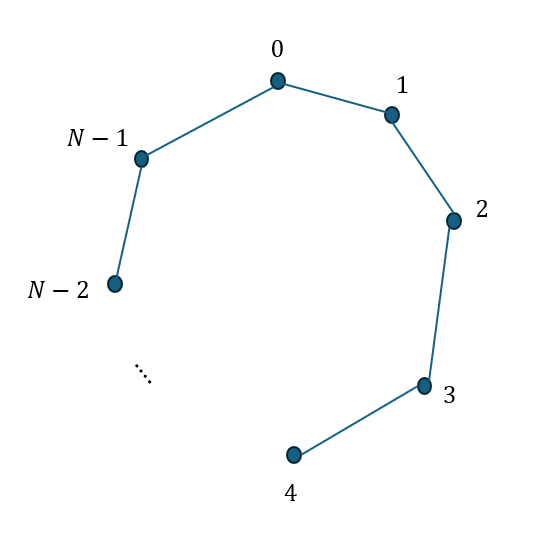
\includegraphics[width=0.5\textwidth]{fig_1.png}  % Replace with your file name
                \caption{Cayley graph of $\mathbb{Z}_N$ with generators $\{\pm 1\}$}
                \label{fig:cayley_z6}
            \end{figure}
        \end{figure}
        
       
    \end{textblock*}


\end{frame}




\begin{frame}{Quantum Walks on Cayley Graphs}
    
    \begin{textblock*}{12cm}(0.5cm,1.5cm)
        
        \textit{Cayley Graphs:} \\
        \vspace{0.3cm}
        
        The adjacency matrix of the Cayley graph $\Gamma = (V,E)$ can be expressed as:
        \[ A = \sum_{a \in G} \lambda_a \ket{\hat{a}} \bra{\hat{a}}, \]
        where $\ket{\hat{a}} = \operatorname{QFT_G} \ket{a}$ is the \textit{Quantum Fourier transform (QFT)} of $\ket{a}$. \\
         \vspace{0.5cm}

        \vspace{2cm}
        
        ... But, What is QFT??
    \end{textblock*}


\end{frame}




\begin{frame}{Quantum Fourier Transform (QFT)}
    
    \begin{textblock*}{12cm}(0.5cm,1.5cm)

            
    Let $G$ be an abelian group. The set of characters of $G$, denoted by $\hat{G}$, is the set of homomorphisms $\chi(a, \cdot): G \to \mathbb{C}$ where $a \in G$. If $G \cong \mathbb{Z}_{N_1} \oplus \cdots \oplus \mathbb{Z}_{N_k}$ then the character $\chi(a, \cdot)$ can be explicitly written as
    \[ \chi(a, x) = \omega_{N_1}^{a_1x_1} \cdots \omega_{N_k}^{a_kx_k} \]
            
    where $\omega_M = \exp(2\pi i/ M)$ is a primitive $M$-th root of unity. The Fourier transform of a function $f: G \to \mathbb{C}$ is given by
    \[ \hat{f}(a) = \frac{1}{\sqrt{|G|}} \sum_{x \in G} \chi(a, x) f(x). \]
    The quantum Fourier transform:
    
    \[
        \sum_{g \in G} f(g) \ket{g} \mapsto \sum_{x \in G} \hat{f}(x)\ket{x}
    \]
   


       
    \end{textblock*}


\end{frame}







\begin{frame}{Quantum Walks on Cayley Graphs}
    
    \begin{textblock*}{12cm}(0.5cm,1.5cm)
        
        \textit{Cayley Graphs:} \\
        \vspace{0.3cm}
        
        The adjacency matrix of the Cayley graph $\Gamma = (V,E)$ can be expressed as:
        \[ A = \sum_{a \in G} \lambda_a \ket{\hat{a}} \bra{\hat{a}}, \]
        Where $\ket{\hat{a}} = \operatorname{QFT}_G(\ket{a}) =  \frac{1}{\sqrt{|G|}}\sum_{g \in G}\chi(a,g)\ket{g}$. \\
        The eigenvalues $\lambda_a$ are given by:
        \[ \lambda_a = \sum_{q \in Q} \chi(a, q). \]
        \begin{itemize}
            \item  Note that the eigenvectors $\ket{\hat{a}}$ of $A$ depend only on $G$ and not on the set $Q$.
        \end{itemize}
    
    \end{textblock*}


\end{frame}








\begin{frame}{Quantum Walks on Cayley Graphs}
    
    \begin{textblock*}{12cm}(0.5cm,1.5cm)
        
        \textit{Cayley Graphs:} \\
        \vspace{0.3cm}
        \textit{Proof}:
        \[
        A\ket{\hat{a}} = A.\frac{1}{\sqrt{|G|}}\sum_{y \in G}\chi(a,y)\ket{y} = \frac{1}{\sqrt{|G|}}\sum_{y \in G}\chi(a,y).A\ket{y}
        \]
        \[
        = \frac{1}{\sqrt{|G|}}\sum_{y \in G}\chi(a,y).\sum_{q \in Q}\ket{qy}
        \]
        Consider $\beta = qy$. Then:
        \[
         = \frac{1}{\sqrt{|G|}}\sum_{q \in Q}\chi(a,q)\sum_{\beta}\chi(a,\beta)\ket{\beta} = \sum_{q \in Q}\chi(a,q) . \ket{\hat{a}}
        \]
        \[
         = \lambda_a\ket{\hat{a}}
        \]
    \end{textblock*}
\end{frame}




\begin{frame}{Group Actions}
    
    \begin{textblock*}{12cm}(0.5cm,1.5cm)
        Cayley graphs can also be constructed using \textit{group actions}.\\
        \vspace{0.5cm}
        \textit{Group Actions:}
        \vspace{0.5cm}
                
        For a group $G$ and a set $X$, we say that $G$ \textit{acts on} $X$ if there is a mapping $*: G \times X \to X$ that satisfies the following properties:
        \begin{enumerate}
            \item Compatibility: for every $a, b \in G$ and every $x \in X$, $g * (h * x) = (gh) * x$,
            \item Identity: for the identity $1 \in G$ and every $x \in X$, $1 * x = x$. 
        \end{enumerate}

        \vspace{0.5 cm}
        \begin{itemize}
            \item  We use the notation $(G, X, *)$ to denote a group $G$ acting on a set $X$ through the action $*$.
            \item  A group action is called \textit{regular} if for every $x, y \in X$ there exists a unique $g \in G$ such that $g * x = y$.
        \end{itemize}


    \end{textblock*}

\end{frame}






\begin{frame}{Cayley Graphs with Group Actions}
    \begin{textblock*}{12cm}(0.5cm,1.5cm)

        \begin{figure}
            \begin{figure}[h!]
                \centering
                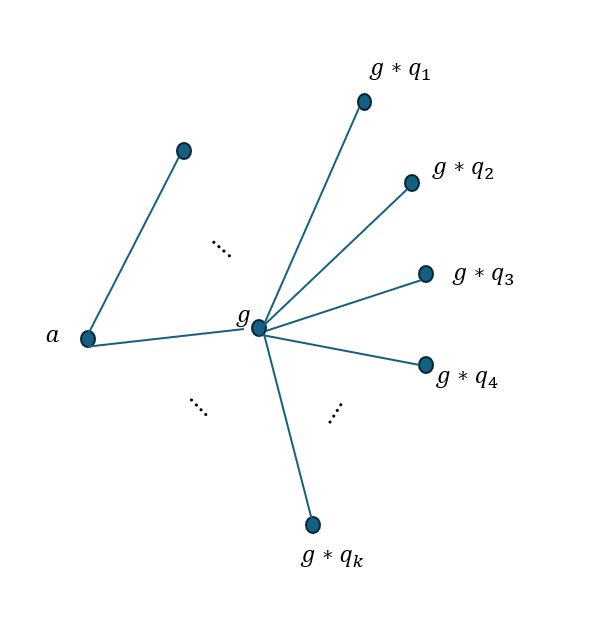
\includegraphics[width=0.5\textwidth]{fig_2.png}  % Replace with your file name
                \caption{Cayley graph of a group $G$ with generators $\{q_1, q_2, ... , q_k\}$}
                \label{fig:cayley_z6}
            \end{figure}
        \end{figure}

    
    \end{textblock*}
\end{frame}






\begin{frame}{Cayley Graphs with Group Actions}
    \begin{textblock*}{12cm}(0.5cm,1.5cm)

    
    Given a regular group action $(G, X, *)$ with a fixed element $x \in X$ and a set  $Q = \{q_1, q_2, \dots, q_k\} \subset G$, let $\Gamma = (X, E)$ be a graphs with vertex set $X$ and edge set consisting of pairs $(x, y) \in X \times X$ such that $y = q * x$ for some $q \in Q$. The adjacency matrix of $\Gamma$ is
    \[
    A = \sum_{h \in G} \lambda_h \ket{G^{(h)} * x} \bra{G^{(h)} * x}, 
    \]
    Where:
    \[
        \ket{G^{(h)} * x} = \frac{1}{\sqrt{|G|}}\sum_{g \in G}\chi(g,h)\ket{g*x}
    \]
    And $\lambda_h = \sum_{q \in Q} \chi(h, q)$. 
    \vspace{0.5cm}
    \begin{itemize}
        \item Again, the eigenvectors $\ket{G^{(h)} * x}$ depend only on $G$.
    \end{itemize}
    \end{textblock*}
\end{frame}






\begin{frame}{Cayley Graphs with Group Actions}
    
    \begin{textblock*}{12cm}(0.5cm,1.5cm)
        \textit{Proof}:

        \[
        A\ket{G^{(h)}*x} = \frac{1}{\sqrt{|G|}}.\sum_{g \in G}\chi(g,h) A.\ket{g*x}
        \]

        \[
        = A\ket{G^{(h)}*x} = \frac{1}{\sqrt{|G|}}.\sum_{g \in G}\chi(g,h)\sum_{q \in Q}\ket{q*(g*x)}
        \]
        Consider $\beta = qg$. Then:
        \[
        = = \frac{1}{\sqrt{|G|}}\sum_{q \in Q}\sum_{\beta \in G}\chi(\beta,h)\chi(q,h)\ket{\beta * x}
        \]

        \[
        = \sum_{q \in Q}\chi(q,h).\ket{G^{(h)}*x} = \lambda_h \ket{G^{(h)}*x}
        \]

    \end{textblock*}

\end{frame}






\begin{frame}{The cmpIndex Algorithm}
    
    \begin{textblock*}{12cm}(0.5cm,1.5cm)
        Given a state $\ket{G^{(h)} * x}$, there is an efficient algorithm for computing $h$.
        Specifically, there is a unitary operator that performs the transformation $\ket{G^{(h)} * x} \ket{0} \mapsto \ket{G^{(h)} * x} \ket{h}$:

        \[
        \ket{G^{(h)} * x}\ket{0} \mapsto \ket{G^{(h)} * x} \frac{1}{\sqrt{|G|}}\sum_{k \in G}\ket{k}
        \]
        And then apply the unitary $\sum_{k \in G}U_k \otimes \ket{k}\bra{k}$:

        \[
        \mapsto \frac{1}{\sqrt{|G|}}\sum_{k \in G}\ket{G^{(h)}*x}\chi(-k,h)\ket{k}
        \]

       
        Finally, applying the inverse quantum Fourier transform to the second register yields:
       

        \[
           \mapsto  \ket{G^{(h)}*x}\ket{h}
        \]
    \end{textblock*}

\end{frame}





\begin{frame}{Simulating continuous-time walks}
    
    \begin{textblock*}{12cm}(0.5cm,1.5cm)
      
        \[
        \ket{\phi_{j0}} := \frac{1}{\sqrt{d}}\sum_{l \in F_j}(\sqrt{\frac{H^*_{jl}}{K}}\ket{0} + \sqrt{1-\frac{|H^*_{jl}|}{K}}\ket{1})
        \]

        \[
        \ket{\phi_{j1}} := \ket{0}\ket{1}
        \]

        \[
        T := \sum_{j=0}^{N-1}\sum_{b \in {\{0,1\}}}(\ket{j}\bra{j}\otimes\ket{b}\bra{b})\otimes\ket{\phi_{jb}}
        \]

        \[
        W = iS(2TT^* - 1)
        \]

        \[
        S\ket{j_1,b_1}\ket{j_2,b_2} = \ket{j_2,b_2}\ket{j_1,b_1}
        \]



    \end{textblock*}

\end{frame}




\begin{frame}{Simulating continuous-time walks}
    
    \begin{textblock*}{12cm}(0.5cm,1.5cm)
      
       \[
       e^{-iAt} = \operatorname{QFT_G}(\sum_{a \in G}e^{-i\lambda_at}\ket{a}\bra{a})\operatorname{QFT^*_G}
       \]




    \end{textblock*}

\end{frame}








% \begin{frame}{Simulating group action quantum walks}
    
%     \begin{textblock*}{12cm}(0.5cm,1.5cm)

%         \[
%         e^{-iAt} = \sum_{h \in G}\ket{G^{(h)}*x}\bra{G^{(h)}*x}
%         \]

%         \[
%         T := \sum_{y \in X}\sum_{b \in {\{0,1\}}}(\ket{j}\bra{j}\otimes\ket{b}\bra{b})\otimes\ket{\phi_{yb}}
%         \]

%         \[
%         = \sum_{y \in X}\sum_{b \in {\{0,1\}}}\ket{y}\ket{b}\ket{\phi_{yb}}\bra{y}\bra{b}
%         \]

%         \[
%             \ket{\phi_{y0}} = \frac{1}{\sqrt{|Q|}}\sum_{q \in Q}\ket{q*y}\ket{0}
%         \]
        

%     \end{textblock*}

% \end{frame}




\begin{frame}{Simulating group action quantum walks}
    
    \begin{textblock*}{12cm}(0.5cm,1.5cm)

        % \begin{align*}
        %     2\ket{0} \bra{0} \otimes TT^* - 1
        %     & = 2\ket{0} \bra{0} \otimes \sum_{y \in X} \sum_{b \in \{0, 1\}} \ket{y, b} \ket{\phi_{yb}} \bra{y, b} \bra{\phi_{yb}} - 1 \\
            
        %     & = U_T (2 \ket{0} \bra{0} \otimes 1_{X, b} \otimes \ket{0, 0} \bra{0, 0} - 1) U_T^*.
        
        % \end{align*}

        \[
        2\ket{0} \bra{0} \otimes TT^* - 1 = 2\ket{0} \bra{0} \otimes \sum_{y \in X} \sum_{b \in \{0, 1\}} \ket{y, b} \ket{\phi_{yb}} \bra{y, b} \bra{\phi_{yb}} - 1 
        \]

        \[
        = 2\sum_{y \in X} \sum_{b \in \{0, 1\}} \ket{0} \ket{y, b} \ket{\phi_{yb}} \bra{0} \bra{y, b} \bra{\phi_{yb}} - 1 
        \]

        \[
        = U_T \Big( 2\sum_{y \in X} \sum_{b \in \{0, 1\}} \ket{0} \ket{y, b} \ket{0, 0} \bra{0} \bra{y, b} \bra{0, 0} - 1 \Big) U_T^* 
        \]

        \[
        = U_T (2 \ket{0} \bra{0} \otimes 1_{X, b} \otimes \ket{0, 0} \bra{0, 0} - 1) U_T^*
        \]

        Now, for any state $\ket{\psi}$:

        \[
        (2\ket{0}\bra{0}\otimes TT^* - 1)\ket{0}\ket{\psi} = \ket{0}(2TT^*-1)\ket{\psi}
        \]

    \end{textblock*}

\end{frame}






\begin{frame}{Group Action Quantum Walks}
    
    \begin{textblock*}{12cm}(0.5cm,1.5cm)
               
        Given a regular group action $(G, X, *)$ with a fixed element $x \in X$ and a set  $Q = \{q_1, q_2, \dots, q_k\} \subset G$, let $\Gamma = (X, E)$ be a graphs with vertex set $X$ and edge set consisting of pairs $(x, y) \in X \times X$ such that $y = q * x$ for some $q \in Q$. The adjacency matrix of $\Gamma$ is
        \[ A = \sum_{h \in G} \lambda_h \ket{G^{(h)} * x} \bra{G^{(h)} * x}, \]
        where:
        \begin{itemize}
            \item $\lambda_h = \sum_{q \in Q} \chi(h, q)$
            \item the eigenvectors $\ket{G^{(h)} * x}$ depend only on $G$
        \end{itemize}

    \end{textblock*}

\end{frame}






\begin{frame}{Application: Quantum Money}
    
    \begin{textblock*}{12cm}(0.5cm,1.5cm)
            
        A public-key quantum money scheme consists of two QPT algorithms:
        \vspace{1cm} 
        \begin{itemize}
        \item $\gen(1^\lambda)$: This algorithm takes a security parameter $\lambda$ as input and outputs a pair $(s, \rho_s)$, where $s$ is a binary string called the serial number, and $\rho_s$ is a quantum state called the banknote. The pair $(s, \rho_s)$, or simply $\rho_s$, is sometimes denoted by $\$$.
        
        \vspace{1cm}
        \item $\ver(s, \rho_s)$: This algorithm takes a serial number and an alleged banknote as input and outputs either $1$ (accept) or $0$ (reject).
        \end{itemize}

    \end{textblock*}


\end{frame}





\begin{frame}{Quantum Money From Group Actions}
    
    \begin{textblock*}{12cm}(0.5cm,1.5cm)
            
        
        \begin{itemize}
        \item $\gen(1^\lambda)$. Begin with the state $\ket{0}\ket{x_\lambda}$, and apply the quantum Fourier transform over $G_\lambda$ to the first register producing the superposition
        \[ \frac{1}{\sqrt{{|X_\lambda|}}} \sum_{g \in G_\lambda} \ket{g}\ket{x_\lambda}. \]
        Next, apply the unitary transformation $\ket{h}\ket{y} \mapsto \ket{h}\ket{h * y}$ to this state, followed by the quantum Fourier transform on the first register. This results in
        \[ \frac{1}{{|G_\lambda|}} \sum_{h \in G_\lambda} \sum_{g \in G_\lambda} \chi(g, h) \ket{h}\ket{g * x_\lambda} = \frac{1}{\sqrt{{|G_\lambda|}}} \sum_{h \in G_\lambda} \ket{h} \ket{G^{(h)} * x_\lambda} \]

        \end{itemize}

        
    \end{textblock*}


\end{frame}




\begin{frame}{Quantum Money From Group Actions}
    
    \begin{textblock*}{12cm}(0.5cm,1.5cm)
            
        
        \begin{itemize}
        \item $\ver(h, \ket{\psi})$. First, check whether $\ket{\psi}$ has support in $X_\lambda$. If not, return $0$. Then, apply $\comph$ to the state $\ket{\psi}\ket{0}$, and measure the second register to obtain some $h' \in G_\lambda$. If $h' = h$, return $1$; otherwise return $0$.
        \end{itemize}

        
    \end{textblock*}


\end{frame}







\begin{frame}{Quantum Money With The Hartley Transform}
    
    \begin{textblock*}{12cm}(0.5cm,1.5cm)
        \textit{Hartley Transform:}\\
        item Let $N$ be a positive integer, and let $\mathbb{Z}_N$ be the additive cyclic group of integers modulo $N$. The Hartley transform of a function $f: \mathbb{Z}_N \to \mathbb{R}$ is the function $\cht_N(f): \mathbb{Z}_N \to \mathbb{R}$ defined by
        \[ \cht_N(f)(a) = \frac{1}{\sqrt{N}} \sum_{y = 0}^{N - 1} \cas\Big(\frac{2 \pi ay}{N}\Big) f(y),  \]
        where $\cas(x) = \cos(x) + \sin(x)$ \\
        For a single basis element of the cyclic group $\mathbb{Z}_N$, the quantum Hartly transform simplifies to
        \begin{equation}
            \label{eq:qht-N}
            \qht_N: \ket{a} \mapsto \frac{1}{\sqrt{N}} \sum_{y = 0}^{N - 1} \cas\Big(\frac{2\pi a y}{N}\Big) \ket{y}.
        \end{equation}
    \end{textblock*}
    

\end{frame}






\begin{frame}{Quantum Money With The Hartley Transform}
    
    \begin{textblock*}{12cm}(0.5cm,1.5cm)
            
        
       
        \begin{itemize}
            \item $\gen$. Begin with the state $\ket{0}\ket{x}$, and apply the quantum Hartley transform over $\mathbb{Z}_N$ to the first register producing the superposition
            \[ \frac{1}{\sqrt{N}} \sum_{g \in \mathbb{Z}_N} \ket{g}\ket{x}. \]
            Next, apply the unitary $\ket{h}\ket{y} \mapsto \ket{h}\ket{h * y}$ to this state, followed by a $\qht_N$ on the first register. This results in
            \[ \frac{1}{N} \sum_{h \in \mathbb{Z}_N} \sum_{g \in \mathbb{Z}_N} \cas\Big(\frac{2\pi gh}{N}\Big) \ket{h}\ket{g * x} = \frac{1}{\sqrt{N}} \sum_{h \in \mathbb{Z}_N} \ket{h} \ket{\mathbb{Z}_N^{(h)} * x}_H \]
            Measure the first register to obtain a random $h \in \mathbb{Z}_N$, collapsing the state to $\ket{\mathbb{Z}_N^{(h)} * x}_H$. Return the pair $(h, \ket{\mathbb{Z}_N^{(h)} * x}_H)$.

        \end{itemize}
        
       
        
    \end{textblock*}


\end{frame}





\begin{frame}{Quantum Money With The Hartley Transform}
    
    \begin{textblock*}{12cm}(0.5cm,1.5cm)
        \begin{itemize}
            \item  In the original scheme, using the quantum Fourier transform, we could directly obtain $h$ from the money state $\ket{\mathbb{Z}_N^{(h)} * x}$ and compare it to the given $h$. However, this approach does not work when we use the Hartley transform. 
            \vspace{1cm}
            \item  To address this, we design an algorithm for computing $h$ that utilizes quantum walks. 

        \end{itemize}
        
        
       
        
    \end{textblock*}


\end{frame}





\begin{frame}{Computing the serial Number}

    \begin{textblock*}{12cm}(0.5cm,1.5cm)

        \begin{itemize}
            \item Given a state $\ket{\mathbb{Z}_N^{(h)} * x}_H$, we show how to compute $h$ using continuous-time quantum walks.
            \vspace{0.5cm}
            \item For any $q \in \mathbb{Z}_N$, define a Cayley graph $\Gamma = (\mathbb{Z}_N, E)$ with the generating set $Q = \{-u, u\}$.
            \vspace{0.5cm}
            \item Let $A$ denote the adjacency matrix of $\Gamma$. The eigenvectors and corresponding eigenvalues of $A$ are $\ket{\mathbb{Z}_N^{(h)} * x}$ and $\lambda_h = 2\cos(2\pi uh / N)$, respectively, for $h \in \mathbb{Z}_N$.
            \vspace{0.5cm}
            \item the unitary $W = e^{iAt}$ can be efficiently simulated to exponential accuracy.
        \end{itemize}


    \end{textblock*}

 \end{frame}



\begin{frame}{Computing the serial Number}

    \begin{textblock*}{12cm}(0.5cm,1.5cm)
        Lemma: The money state $\ket{\mathbb{Z}_N^{(h)} * x}_H$ is an eigenstate of $W$ with eigenvalue $e^{i\lambda_h t}$.
        % \vspace{1cm}
        

        \textit{Proof:}
        \begin{align*}
            e^{iAt} \ket{\mathbb{Z}_N^{(h)} * x}_H
            & = \sum_{g \in \mathbb{Z}_N} e^{i\lambda_gt} \ket{\mathbb{Z}_N^{(g)} * x}\braket{\mathbb{Z}_N^{(g)} * x|\mathbb{Z}_N^{(h)} * x}_H 
        \end{align*}


        \[
        =\sum_{g \in \mathbb{Z}_N} e^{i\lambda_gt} \ket{\mathbb{Z}_N^{(g)} * x} \bra{\mathbb{Z}_N^{(g)} * x} \Big( \frac{1 - i}{2} \ket{\mathbb{Z}_N^{(h)} * x} + \frac{1 + i}{2} \ket{\mathbb{Z}_N^{(-h)} * x} \Big) 
        \]

        \[
        =e^{i\lambda_{h}t} \frac{1 - i}{2} \ket{\mathbb{Z}_N^{(h)} * x} + \frac{1 + i}{2} e^{i\lambda_{-h}t} \ket{\mathbb{Z}_N^{(-h)} * x} 
        \]


        \[
        =e^{i\lambda_{h}t} \ket{\mathbb{Z}_N^{(h)} * x}_H,
        \]


        where the last equality follows from the fact that $\lambda_h = \lambda_{-h}$.
    \end{textblock*}

 \end{frame}



 
\begin{frame}{Computing the serial Number}

    \begin{textblock*}{12cm}(0.5cm,1.5cm)
        Lemma: The money state $\ket{\mathbb{Z}_N^{(h)} * x}_H$ is an eigenstate of $W$ with eigenvalue $e^{i\lambda_h t}$.
        \vspace{1cm}

        $e^{iAt} \ket{\mathbb{Z}_N^{(h)} * x}_H$ = $e^{i\lambda_{h}t} \ket{\mathbb{Z}_N^{(h)} * x}_H$
        
        \vspace{1cm}
        If we choose $t = \operatorname{poly}(\log N)$, it follows from Lemma that we can run the \textit{phase estimation algorithm} with the unitary $W$ and the eigenstate $\ket{\mathbb{Z}_N^{(h)} * x}_H$ to compute an estimate $\tilde{\lambda}_h$ of $\lambda_h$ such that %$\abs{\tilde{\lambda}_h - \lambda_h} \le 1 / poly(log N)$. 
        % \operatorname{poly}(\log N)
        \[
        |\tilde{\lambda}_h - \lambda_h| \leq \frac{1}{\operatorname{poly}(\log N)}
        \]
        

        
    \end{textblock*}

 \end{frame}




\begin{frame}{An efficient new algorithm for QHT}
    
    \begin{textblock*}{12cm}(0.5cm,1.5cm)
        Now, let us briefly explain how the algorithm for $\qft_N$ works:
        \begin{align*}
            \qft_N\ket{a}
            & = \frac{1}{\sqrt{N}} \sum_{y = 0}^{N - 1} \omega_N^{ay}\ket{y} \\
            & = \frac{1}{\sqrt{N}} \sum_{y = 0}^{N / 2 - 1} \omega_N^{ay} \ket{y} + (-1)^a \sum_{y = 0}^{N / 2 - 1} \omega_N^{ay} \ket{y + N/2} \\
            & = \frac{1}{\sqrt{N / 2}} \sum_{y = 0}^{N / 2 - 1} \omega_N^{ay} \frac{1}{\sqrt{2}} (\ket{0} + (-1)^a \ket{1}) \ket{y}, \numberthis\label{eq:qft_alt}
        \end{align*}
       
    \end{textblock*}
    

\end{frame}


\begin{frame}{An efficient new algorithm for QHT}
    
    \begin{textblock*}{12cm}(0.5cm,1.5cm)
        Let $\ket{a} = \ket{t}\ket{b}$, where $b$ is the least significant bit of $a$, so that $a = 2t + b$. Applying $\qft_{N / 2}$ to the first register, we obtain the state
        \[ \frac{1}{\sqrt{N / 2}} \sum_{y = 0}^{N / 2 - 1} \omega_N^{2ty} \ket{y} \ket{b}. \]
        Next, we apply the phase unitary $P(y, b): \ket{y} \ket{b} \mapsto \omega_N^{by} \ket{y} \ket{b}$, and finally, we apply a Hadamard transform to the last qubit. The result is the state in \eqref{eq:qft_alt}.  

    \end{textblock*}
    

\end{frame}



\begin{frame}{An efficient new algorithm for QHT}
    
    \begin{textblock*}{12cm}(0.5cm,1.5cm)
        \begin{equation}
            % \label{eq:cas-expand}
            \frac{1}{\sqrt{N}} \sum_{y = 0}^{N - 1} \cas\Big( \frac{2\pi a y}{N} \Big) \ket{y}  
        \end{equation}
        \begin{equation}
            = \frac{1}{\sqrt{N}} \sum_{y = 0}^{N / 2 - 1} \cas\Big( \frac{2\pi a y}{N} \Big) \ket{y} +  \frac{1}{\sqrt{N}} \sum_{y = N / 2}^{N - 1} \cas\Big( \frac{2\pi a y}{N} \Big) \ket{y}.
        \end{equation}
        The second sum in the right-hand side can be written as 
        \begin{align*}
            \sum_{y = N / 2}^{N - 1} \cas\Big( \frac{2\pi a y}{N} \Big) \ket{y}
            & = \sum_{y = 0}^{N / 2 - 1} \cas\Big( \frac{2\pi a y}{N} + \pi a \Big) \ket{y + N/2} \\
            & = (-1)^a \sum_{y = 0}^{N / 2 - 1} \cas\Big( \frac{2\pi a y}{N} \Big) \ket{y + N/2},
        \end{align*}
    \end{textblock*}

\end{frame}




\begin{frame}{An efficient new algorithm for QHT}
    
    \begin{textblock*}{12cm}(0.5cm,1.5cm)
       
        \begin{align}
            % \frac{1}{\sqrt{N}} \sum_{y = 0}^{N - 1} \cas\Big( \frac{2\pi a y}{N} \Big) \ket{y}
            % & = \frac{1}{\sqrt{N}} \sum_{y = 0}^{N / 2 - 1} \cas\Big( \frac{2\pi a y}{N} \Big) (\ket{y} + (-1)^a \ket{y + N/2}) \nonumber \\
            & = \frac{1}{\sqrt{N / 2}} \sum_{y = 0}^{N / 2 - 1} \cas\Big( \frac{2\pi a y}{N} \Big) \frac{1}{\sqrt{2}} (\ket{0} + (-1)^a \ket{1}) \ket{y}, \label{eq:qht-alt} 
        \end{align}

        We now show how to compute $\qht_N$ recursively.

        \begin{align*}
            \ket{0}\ket{t}\ket{b}
            & \mapsto \frac{1}{\sqrt{N / 2}} \sum_{y = 0}^{N / 2 - 1} \cas\Big( \frac{2\pi t y}{N / 2} \Big) \ket{0} \ket{y} \ket{b} \\%& (\mathds{1} \otimes \qht_{N / 2} \otimes \mathds{1}) \\
            & = \frac{1}{\sqrt{N / 2}} \sum_{y = 0}^{N / 2 - 1} \cas\Big( \frac{4\pi t y}{N} \Big) \ket{0} \ket{y} \ket{b} \\
            & \mapsto \frac{1}{\sqrt{N}} \sum_{y = 0}^{N / 2 - 1} \cas\Big( \frac{4\pi t y}{N} \Big) (\ket{0} + \ket{1}) \ket{y}\ket{b}. %& (H \otimes \mathds{1}) 
        \end{align*}
        
    \end{textblock*}
    
\end{frame}



% \begin{frame}{An efficient new algorithm for QHT}
    
%     \begin{textblock*}{12cm}(0.5cm,1.5cm)
       
%         \begin{align}
%             % \frac{1}{\sqrt{N}} \sum_{y = 0}^{N - 1} \cas\Big( \frac{2\pi a y}{N} \Big) \ket{y}
%             % & = \frac{1}{\sqrt{N}} \sum_{y = 0}^{N / 2 - 1} \cas\Big( \frac{2\pi a y}{N} \Big) (\ket{y} + (-1)^a \ket{y + N/2}) \nonumber \\
%             & = \frac{1}{\sqrt{N / 2}} \sum_{y = 0}^{N / 2 - 1} \cas\Big( \frac{2\pi a y}{N} \Big) \frac{1}{\sqrt{2}} (\ket{0} + (-1)^a \ket{1}) \ket{y}, \label{eq:qht-alt} 
%         \end{align}

%         We now show how to compute $\qht_N$ recursively.

%         \begin{align*}
%             \ket{0}\ket{t}\ket{b}
%             & \mapsto \frac{1}{\sqrt{N / 2}} \sum_{y = 0}^{N / 2 - 1} \cas\Big( \frac{2\pi t y}{N / 2} \Big) \ket{0} \ket{y} \ket{b} \\%& (\mathds{1} \otimes \qht_{N / 2} \otimes \mathds{1}) \\
%             & = \frac{1}{\sqrt{N / 2}} \sum_{y = 0}^{N / 2 - 1} \cas\Big( \frac{4\pi t y}{N} \Big) \ket{0} \ket{y} \ket{b} \\
%             & \mapsto \frac{1}{\sqrt{N}} \sum_{y = 0}^{N / 2 - 1} \cas\Big( \frac{4\pi t y}{N} \Big) (\ket{0} + \ket{1}) \ket{y}\ket{b}. %& (H \otimes \mathds{1}) 
%         \end{align*}
        
%     \end{textblock*}
    

% \end{frame}




\begin{frame}{An efficient new algorithm for QHT}
    
    \begin{textblock*}{12cm}(0.5cm,1.5cm)

        
        \begin{algorithm}[${QHT}_N$] 
            \begin{itemize}
                \item   Input: quantum state $\ket{\psi} \in \mathbb{C}^N$, where $N = 2^n$
                \item   Output: quantum state $\qht_N\ket{\psi}$ 
            \end{itemize}
        \end{algorithm}
    \end{textblock*}

        \begin{textblock*}{12cm}(0.5cm,4cm)
            1- Initialize an ancilla qubit to $0$ to obtain the state $\ket{0}\ket{\psi}$ \\
            2-  Compute ${1} \otimes \qht_{N / 2} \otimes {1}$ recursively.\\
            3-  Apply $H \otimes {1}$.\\
            4-  Apply  the controlled negation $\ket{0}\ket{y} \mapsto \ket{0}\ket{y}, \ket{1}\ket{y} \mapsto \ket{1}\ket{N / 2 -y}$ to the first two registers.\\
            5-  Apply the unitary $U_R$.\\
            6-  Apply $H \otimes {1}$\\
            7-  Apply \textsc{cnot} to the first and last qubits.\\
            8-  Apply ${1} \otimes H$.\\
            9-  Trace out the first qubit
        \end{textblock*}
        

\end{frame}






\begin{frame}{References}
    
    \begin{textblock*}{12cm}(0.5cm,1.5cm)

        
    \end{textblock*}
        

\end{frame}




 

% End
\end{document}


    